\chapter{Data Warehousing}\label{cha:datawarehousing}

\section{Was ist ein DWH?}

Ein Data Warehouse (deutsch: Datenlager) ist ein System, das Daten aus vielen verschiedenen Quellen für die Berichterstellung und Analyse zusammenführt.
Die aus komplexen Abfragen in einem Data Warehouse erstellten Berichte werden verwendet, um Geschäftsentscheidungen zu treffen.

Der Inhalt von Data Warehouses entsteht durch Kopieren, Sammeln, Transformieren und sonstigem Aufbereiten von Daten aus unterschiedlichen Quellen.
Der Zweck eines Data Warehouse besteht darin,
\begin{itemize}
    \item Daten, die auf verschiedene Dateninseln verteilt existieren, in einer konsistenten Datensammlung zusammenzufassen,
    \item Die Vielzahl der unstrukturierten Informationen so aufzubereiten, dass neues Wissen entsteht.
\end{itemize}

Die Kombination eines Data Warehouse mit OLAP-Techniken macht aus den Daten wertvolle Informationen, die sich auf einfache Weise auswerten lassen.

\section{Unterschied DWH und Datenbank}

Data Warehouses und Datenbanken sind beides relationale Datensysteme, jedoch wurden beide für unterschiedliche Zwecke erstellt. Ein Data Warehouse ist so aufgebaut, dass große Mengen an historischer Daten gespeichert werden und schnelle, komplexe Abfragen für alle Daten möglich sind, normalerweise mithilfe von OLAP. Eine Datenbank wurde erstellt, um aktuelle Transaktionen zu speichern und einen schnellen Zugriff auf bestimmte Transaktionen für laufende Geschäftsprozesse zu ermöglichen, dies geschieht jedoch mit OLTP.

\section{Charakteristiken eines DWH}

\begin{itemize}
    \item Fachorientierung (subject-oriented):
    \begin{itemize}
        \item Zweck des Systems ist nicht Erfüllung einer Aufgabe sondern Modellierung eines spezifischen Anwendungsziels
    \end{itemize}
    \item Integrierte Datenbasis (integrated):
    \begin{itemize}
        \item Verarbeitung von Daten aus mehreren verschiedenen Datenquellen (intern und extern)
    \end{itemize}
    \item Nicht-flüchtige Datenbasis (non-volatile):
    \begin{itemize}
        \item stabile, dauerhafte Datenbasis
        \item Daten im Data Warehouse werden nicht mehr entfernt oder geändert       
    \end{itemize}
    \item Historische Daten (time-variant):
    \begin{itemize}
        \item Vergleich der Daten über Zeit möglich
        \item Speicherung über längeren Zeitraum
    \end{itemize}
\end{itemize}

\section{ETL}

Der ETL-Prozess beschreibt den Extraktion-Transformation-Lade-Prozess und besteht aus folgenden Schritten:
\begin{itemize}
    \item Datenbeschaffung: d.h. Extraktion der relevanten Daten aus den Quellsystemen und Bereitstellung der Daten in einem Arbeitsbereich (engl. staging area)
    \item Transformation für die Strukturanpassung und ggf. Bereinigung der Daten (engl. data cleaning resp. data cleansing) im Arbeitsbereich
    \item Laden der Daten aus dem Arbeitsbereich in das zentrale Datenlager, das Data Warehouse
\end{itemize}

\section{Referenzmodell der DWH Architektur}

\begin{figure}[H]
    \centering
    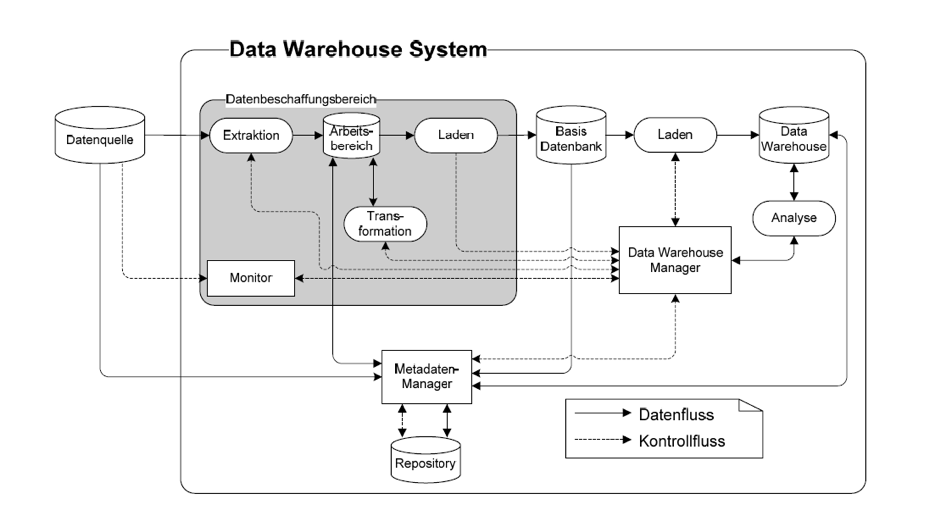
\includegraphics[width=0.5\textwidth]{Content/images/dwh/dwh.png}
    \caption{Referenzmodell der DWH Architektur}
    \label{fig:dwh:dwh}
\end{figure}

\subsection{Phasen des DWH}

\begin{enumerate}
    \item Überwachen der Datenquellen (stellen die Lieferanten der Daten für das Data Warehouse dar, gehören nicht direkt zum DWH) auf Änderungen durch die Monitore
    \item Kopieren der relevanten Daten mittels Extraktion in den temporären Arbeitsbereich
    \item Transformation der Daten im Arbeitsbereich (Bereinigung, Integration)
    \item Kopieren der Daten in integrierte Basisdatenbank als Grundlage für verschiedene Analysen
    \item Laden der Daten in das Data Warehouse

\end{enumerate}

\subsection{Monitore}

Monitore haben die Aufgabe Datenmanipulationen in einer Datenquelle zu erkennen und diese zu melden, dabei gibt es folgende Strategien:

\begin{itemize}
    \item Triggerbasiert: wenn Datenbankänderungen auftreten, werden die geänderten Tupel in einen anderen Bereich kopiert
    \item Replikationsbasiert: geänderte Tupel werden in spezielle Tabellen geschrieben
    \item Zeitstempelbasiert: jedem Datensatz wird ein Zeitstempel zugeordnet dadurch können geänderte Datensätze identifiziert werden
    \item Logbasiert: hier werden die Log-Dateien der Transaktionen verwendet um Änderungen zu erkennen
    \item Snapshotbasiert: bei dieser Strategie werden periodische Kopien des Datenbestandes in Dateien abgelegt (Snapshot) Aufgrund des Vergleichs von Snapshots können anschließend Änderungen erkannt werden
\end{itemize}

\subsection{Arbeitsbereich}

Er stellt die zentrale Datenhaltungskomponente des Datenschaffungsbereiches dar und dient als Temporärer Zwischenspeicher zur Integration. Weiters werden auf ihm Transformationen ausgeführt (fungiert wie eine Art Cache).

\subsection{Extraktion}

Die Extraktion hat die Aufgabe, Daten aus den Quellen in den Arbeitsbereich zu übertragen. Dazu werden Standardschnittstellen wie z.B.: ODBC verwendet.

\subsection{Transformation}

Die Transformationskomponente hat folgende Aufgaben:
\begin{itemize}
    \item Vorbereitung und Anpassung der Daten für das Laden
    \item Überführung aller Daten in ein einheitliches Format
    \item Beseitigung von Verunreinigungen
    \item Angleichen der Abtastfrequenz
\end{itemize}

\subsection{Ladekomponente}

Die Ladekomponente dient der Übertragung der von der Transformation aufbereiteten Daten in die Basisdatenbank bzw. In das DWH.

\subsection{Basisdatenbank}

Die Basisdatenbank dient für konkrete Analysen der Datenbasis und versorgt das Data Warehouse mit bereinigten Daten. 

\subsection{Repository}

Das Repository übernimmt die Speicherung der Metadaten des DWH-Systems. Metadaten sind Informationen, die den Aufbau, die Wartung und Administration des DW-Systems vereinfachen und die Informationsgewinnung ermöglichen. (Beispiel: Datenbankschemata, Zugriffsrechte, Prozessinformationen)

\subsection{Metadaten Manager}

Er hat die Aufgabe, die Metadaten- sowie eine Versions- und Konfigurationsverwaltung zu organisieren.

\section{Data Marts}

Ein Data Mart ist ein Auszug (ganze oder teilweise Kopie) aus einem Data Warehouse oder eine Sicht auf das Data Warehouse (View) für einen bestimmten Organisationsbereich oder eine bestimmte Anwendung.
Gründe hierfür - anstelle des direkten Arbeitens mit den Daten im Data Warehouse - können beispielsweise sein:
\begin{itemize}
    \item spezielle Datenstrukturen, z.B. für die mehrdimensionale Analyse, das sog. Online Analytical Processing (OLAP)
    \item bessere Leistung (Performance): Verlagerung von Rechnerleistung auf einen anderen Rechner und/oder Verlagerung von Zugriffen auf einen anderen Speicher
    \item mehr Zugriffsschutz: Abgrenzung gegenüber anderen Nutzern oder Öffnung für weitere Nutzer.
\end{itemize}

\begin{figure}[H]
    \centering
    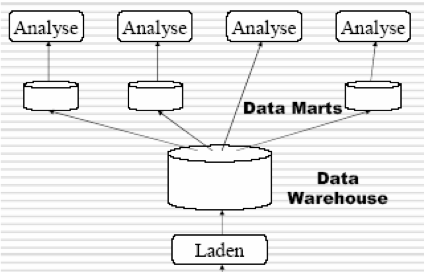
\includegraphics[width=0.4\textwidth]{Content/images/dwh/mart.png}
    \caption{Data Mart}
    \label{fig:dwh:mart}
\end{figure}

\section{Analysewerkzeuge}

Sie dienen der Auswertung bzw. Analyse der gesammelten Daten sowie der Aufbereitung der Ergebnisse für die Weiterverarbeitung.
Analysewerkzeuge:
\begin{itemize}
    \item OLAP und OLTP
    \item Data Mining
\end{itemize}

\subsection{OLAP und OLTP}

In der Online Datenverarbeitung gibt es grundsätzlich zwei Arten: OnLine Transaction Processing und OnLine Analytical Processing.

OLTP bezieht sich auf die Vorgänge bei denen Daten gelesen, geschrieben, bzw. Upgedatet werden (findet in operationellen Systemen).

Bsp.:
Kunde kommt in eine Bank und betätigt eine Buchung, nun werden in seinem Konto Daten gelesen und upgedatet.

OLAP ist kein operationeller Prozess sonder analysiert bereits vorhandenen Daten.
Durch OLAP werden Verbindungen zwischen auf den ersten Blick unabhängigen Daten gefunden. Dies geschieht durch multidimensionale Datenanalyse
Weiters hat OLAP folgende Anforderungen:
\begin{itemize}
    \item multidimensionale Sicht auf die Daten
    \item transparenter Zugang zu Datenbeständen mit logischer Gesamtsicht
    \item stabile, volumenunabhängige Antwortzeiten
    \item Skalierbarkeit auf große Datenmengen
    \item unbegrenzte Anzahl an Dimensionen und Aggregationsebenen
    \item unbeschränkte dimensionsübergreifende Operationen
    \item Mehrbenutzerunterstützung
\end{itemize}

\begin{figure}[H]
    \centering
    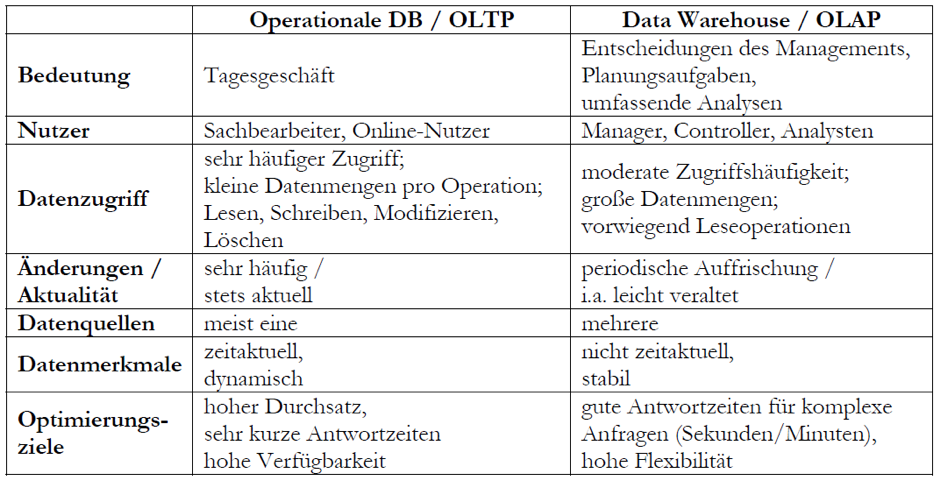
\includegraphics[width=0.67\textwidth]{Content/images/dwh/oltp.png}
    \caption{OLTP}
    \label{fig:dwh:oltp}
\end{figure}

\subsection{Data Mining}

Unter Data-Mining versteht man die systematische Anwendung statistischer Methoden auf große Datenbestände mit dem Ziel, neue Querverbindungen, Regeln, Beziehungsmuster, Abhängigkeiten und Trends zu erkennen. 
In der Praxis wurde der Unterbegriff Data-Mining auf den gesamten Prozess der sogenannten „Knowledge Discovery in Databases“ (englisch für Wissensentdeckung in Datenbanken; KDD) übertragen, der auch Schritte wie die Vorverarbeitung und Auswertung beinhaltet, während Data-Mining im engeren Sinne nur den eigentlichen Verarbeitungsschritt des Prozesses bezeichnet.

\begin{figure}[H]
    \centering
    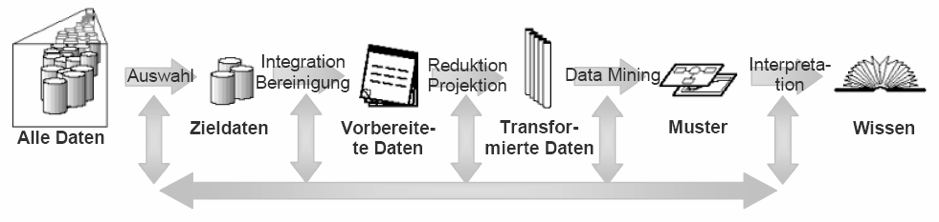
\includegraphics[width=0.8\textwidth]{Content/images/dwh/mining.png}
    \caption{Data Mining}
    \label{fig:dwh:mining}
\end{figure}

\section{Multidimensionale Datenstruktur}

Im Vergleich zu relationalen Datenbanken, welche Daten in Zeilen und Spalten abspeichern speichern OLAP-Datenbanken Datensätze mehrdimensional ab.

\begin{figure}[H]
    \centering
    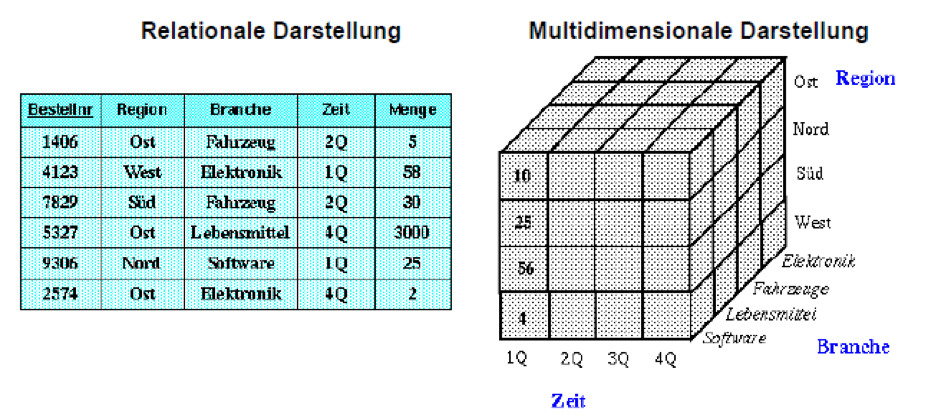
\includegraphics[width=.5\textwidth]{Content/images/dwh/multi.png}
    \caption{}
    \label{fig:dwh:multi}
\end{figure}

Bsp.:
In einem Unternehmen wird ein DWH eingesetzt. Nun interessieren sich aber die Arbeiter der verschiedenen Abteilungen für verschiedene Bezugsgrößen.
So interessiert sich etwa ein Produktmanager für die Verkaufszahlen eines Produkts in allen Absatzgebieten über sämtliche Monate eines Jahres hinweg, während ein Gebietsleiter Angaben zu allen Produkten und Monaten für ein bestimmtes Gebiet benötigt.

Hier sind Produkt, Zeit und Gebiet die verschiedenen Dimensionen. Elemente der einzelnen Dimensionen bezeichnet man als Ausprägungen (engl. Members). Für die Dimension Gebiet könnte zum Beispiel "Oberösterreich" eine Ausprägung darstellen.

Darüber hinaus muss sich der Maßstab jeder Dimension skalierbar sein. So will z.B. ein Produktmanager nicht an Monate als Betrachtungszeiträume gebunden sein, sondern bei Bedarf auch die Werte pro Woche oder Jahr anschauen, d.h. es muss eine Dimensions-Hierarchie vorhanden sein:

\section{Star- und Snowflake Schema}

\begin{wrapfigure}{r}{0.5\textwidth}
    \begin{center}
      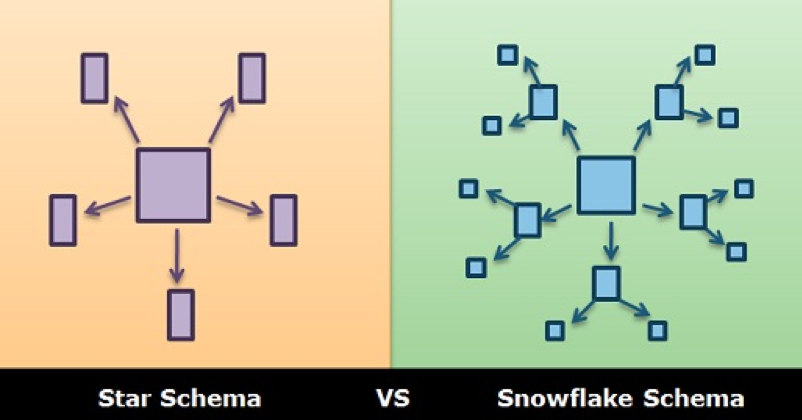
\includegraphics[width=0.48\textwidth]{Content/images/dwh/starsnow.png}
    \end{center}
    \caption{}
  \end{wrapfigure}
  Stern- und Schneeflockenschemata sind die beliebtesten mehrdimensionalen Datenmodelle, die für ein Data Warehouse verwendet werden. Der entscheidende Unterschied zwischen dem Sternschema und dem Schneeflockenschema besteht darin, dass das Sternschema keine Normalisierung verwendet, während das Schneeflockenschema eine normalisiertes Datensystem verwendet, um die Redundanz von Daten zu beseitigen. Fakten- und Dimensionstabellen sind wesentliche Voraussetzungen für die Erstellung eines Schemas.

  \subsection{Starschema}

  Das Sternschema ist das einfache und allgemeine Modellierungsparadigma, bei dem das Data Warehouse eine Faktentabelle mit einer einzelnen Tabelle für jede Dimension enthält. Das Schema imitiert einen Stern, wobei die Dimensionstabelle in einem übergeordneten Muster dargestellt wird, das die zentrale Faktentabelle umgibt. Die Dimensionstabelle wird über Primärschlüssel und Fremdschlüssel mit der Dimensionstabelle verbunden.

  Beispiel:

  \begin{wrapfigure}{r}{0.5\textwidth}
    \begin{center}
      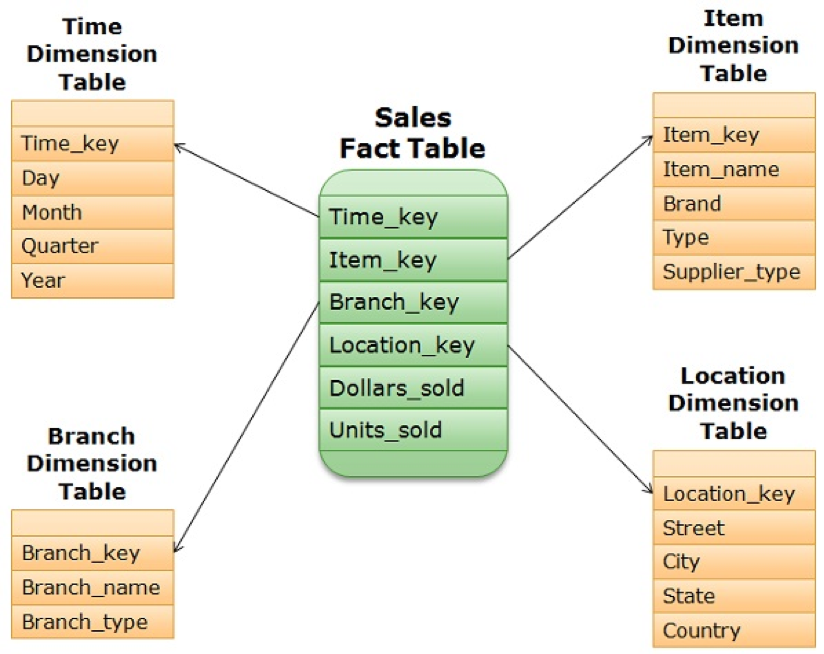
\includegraphics[width=0.48\textwidth]{Content/images/dwh/star.png}
    \end{center}
    \caption{Star Schema}
  \end{wrapfigure}
  Nur eine einzelne Tabelle imitiert jede Dimension, und jede Tabelle enthält eine Gruppe von Attributen, wie sie im Sternschema angezeigt werden. Die Standortdimensionstabelle umfasst den Attributsatz (locationkey, street, city, state und country). Diese Einschränkung kann zu Redundanz führen. Beispielsweise können zwei Städte denselben Bundesstaat und dasselbe Land haben. Daher führen Einträge für solche Städte in der Standortdimensionstabelle zu einer Redundanz zwischen den Bundesstaat- und Länderattributen.

  \subsection{Snowflake Schema}

  Das Schneeflockenschema ist die Art des Sternschemas, welches die hierarchische Form von Maßtabellen enthält. In diesem Schema gibt es eine Faktentabelle mit verschiedenen Dimensionen und Unterdimensionstabellen, die über Primär- und Fremdschlüssel mit der Faktentabelle verbunden sind. Sie wird Schneeflocke genannt, weil ihre Struktur einer Schneeflocke ähnelt.

  Es wird eine Normalisierung verwendet, die die Daten in zusätzliche Tabellen aufteilt. Die Aufteilung führt zu einer Verringerung der Redundanz und zur Vermeidung von Speicherverlusten. Ein Schneeflockenschema ist einfacher zu verwalten, aber komplex zu entwerfen und zu verstehen. Dies kann auch die Effizienz des Browsens verringern, da zum Ausführen einer Abfrage mehr Joins erforderlich sind.
  
\begin{figure}[H]
    \centering
    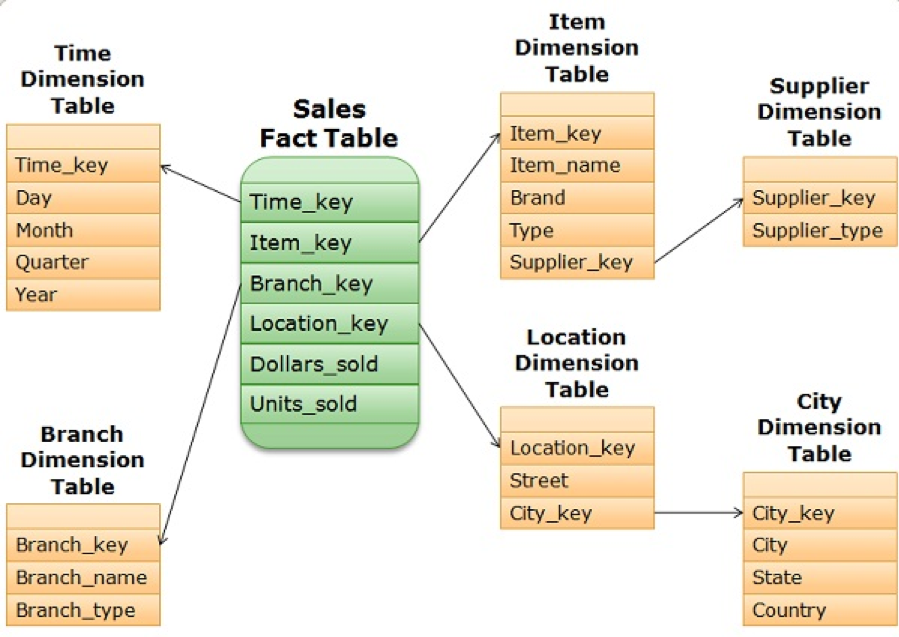
\includegraphics[width=0.5\textwidth]{Content/images/dwh/snow.png}
    \caption{}
\end{figure}

Beispiel:
In ähnlicher Weise enthält die Standortdimensionstabelle die Attribute locationkey, street und citykey, und citykey sind mit der Stadtdimensionstabelle verknüpft, die das Attribut city, state und country enthält. Hier kann auch das Zustandsattribut weiter normalisiert werden.

\subsection{Unterschiede}

\begin{enumerate}
    \item Das Sternschema enthält nur eine Dimensionstabelle für einen Dimensionseintrag, während für einen Eintrag möglicherweise eine Dimension und eine Unterdimensionstabelle vorhanden sind.
    \item Die Normalisierung wird im Schneeflockenschema verwendet, wodurch die Datenredundanz beseitigt wird. Im Gegensatz dazu wird die Normalisierung nicht im Sternschema durchgeführt, was zu Datenredundanz führt.
    \item Sternschema ist einfach, leicht zu verstehen und beinhaltet weniger komplizierte Abfragen. Im Gegenteil, Schneeflockenschemata sind schwer zu verstehen und beinhalten komplexe Abfragen.
    \item Der in einem Sternschema verwendete Datenmodellansatz ist top-down, während das Schneeflockenschema bottom-up verwendet.
    \item Das Sternschema verwendet weniger Joins. Andererseits verwendet das Schneeflockenschema eine große Anzahl von Verknüpfungen.
    \item Der vom Sternschema belegte Speicherplatz ist im Vergleich zum Schneeflockenschema größer.
    \item Der Zeitaufwand für die Ausführung einer Abfrage in einem Sternschema ist geringer. Umgekehrt nimmt das Schneeflockenschema aufgrund der übermäßigen Verwendung von Verknüpfungen mehr Zeit in Anspruch.
    
\end{enumerate}

\section{Cube Operationen}

\subsection{Drill Down}

Hier steigt man von der jeweiligen Dimensionsebene auf die nächst tiefere

\begin{figure}[H]
    \centering
    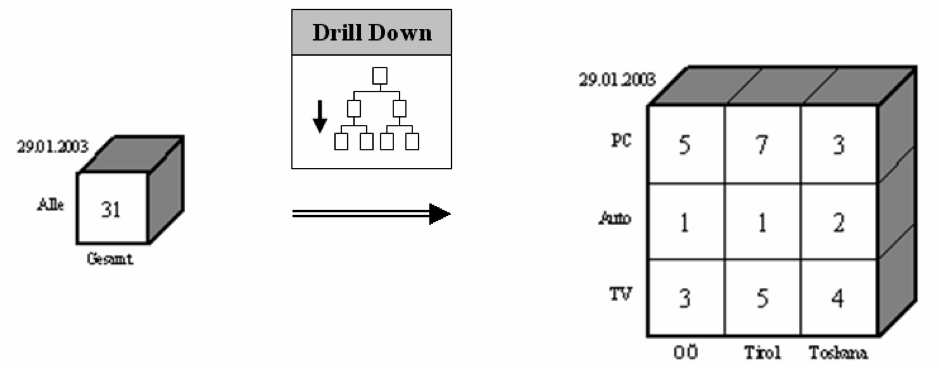
\includegraphics[width=0.5\textwidth]{Content/images/dwh/drill.png}
    \caption{}
\end{figure}

\subsection{Roll Up}

Umkehr-Operation zu Drill Down
\begin{figure}[H]
    \centering
    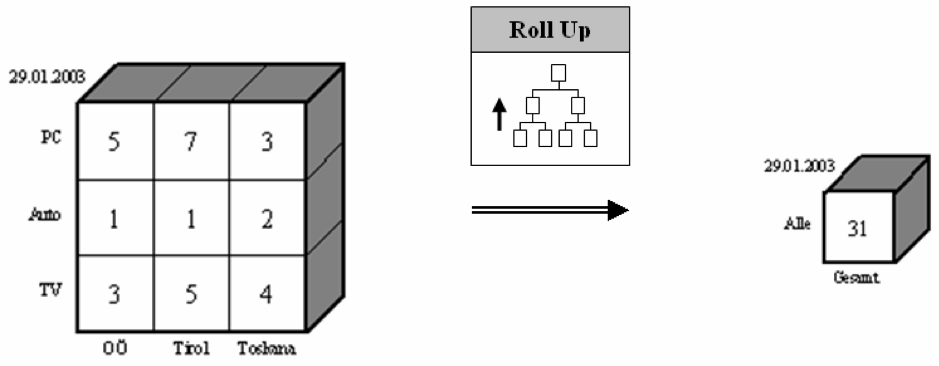
\includegraphics[width=0.5\textwidth]{Content/images/dwh/rollup.png}
    \caption{}
\end{figure}

\subsection{Slice}

Hier schneidet man eine Scheibe aus dem sogenannten dreidimensionalen Hypercube. Diese Operation ergibt eine zweidimensionale Matrix.
\begin{figure}[H]
    \centering
    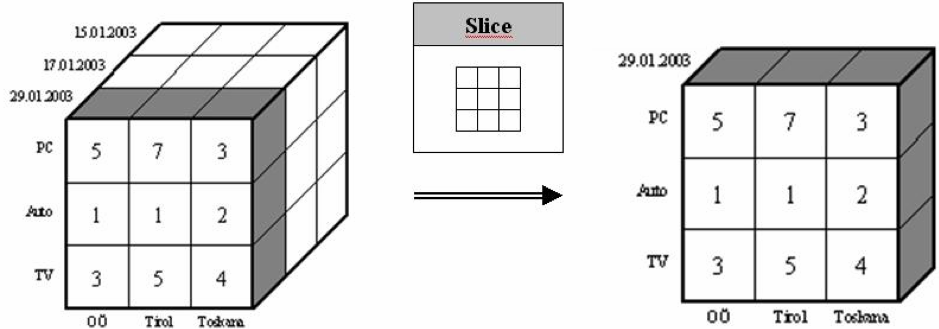
\includegraphics[width=0.5\textwidth]{Content/images/dwh/slice.png}
    \caption{}
\end{figure}

\subsection{Dice}

Bei dieser Operation wird ein Teilwürfel des Hypercubes herausgeschnitten.
\begin{figure}[H]
    \centering
    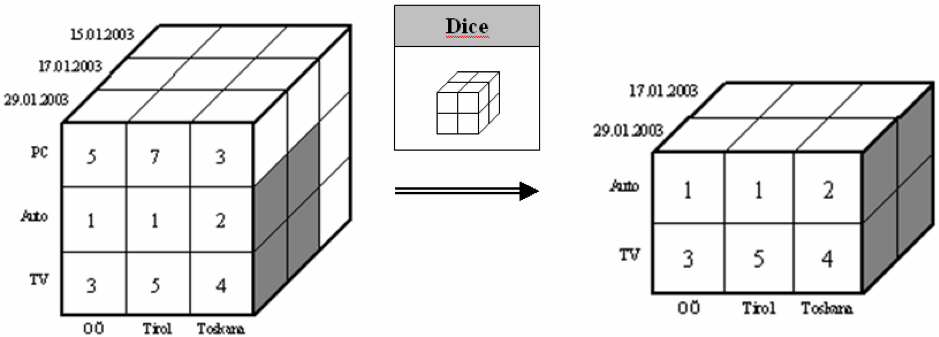
\includegraphics[width=0.5\textwidth]{Content/images/dwh/dice.png}
    \caption{}
\end{figure}

\subsection{Rotate}

Diese Operation Rotiert den Hypercube um eine andere Sichtweise auf die Daten zu erlangen.
\begin{figure}[H]
    \centering
    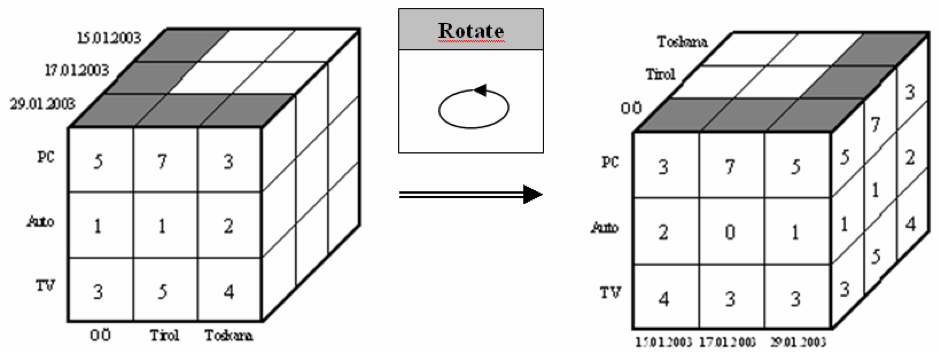
\includegraphics[width=0.5\textwidth]{Content/images/dwh/rotate.png}
    \caption{}
\end{figure}

\subsection{Nest}

Mit dieser Operation kann man einen dreidimensionalen Bereich des Hypercubes in einer zweidimensionale Matrix darstellen.
\begin{figure}[H]
    \centering
    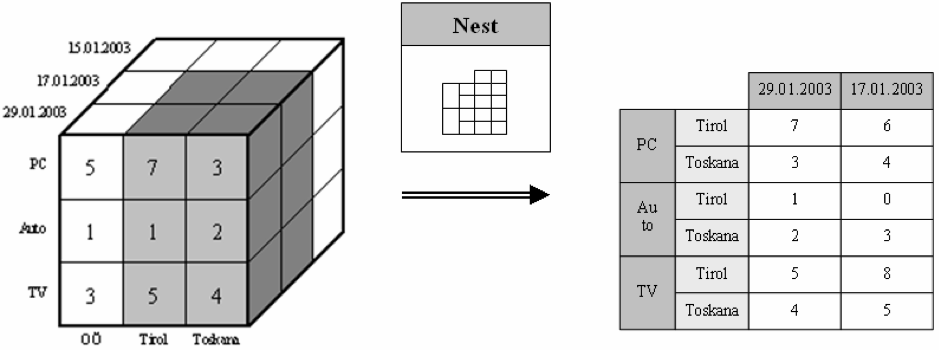
\includegraphics[width=0.5\textwidth]{Content/images/dwh/nest.png}
    \caption{}
\end{figure}
\begin{figure}[H]
    \centering
    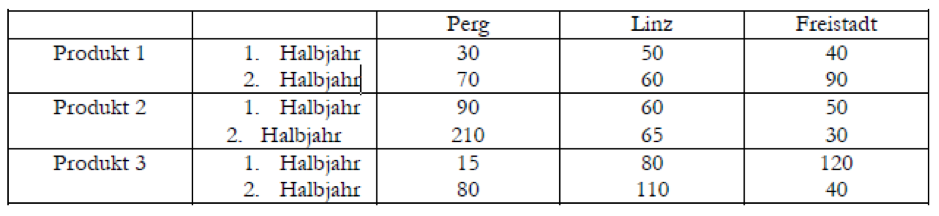
\includegraphics[width=0.5\textwidth]{Content/images/dwh/table.png}
    \caption{}
\end{figure}

